\section{Un arbre pondéré est donné (7 points)}

\emph{Les résulats approchés sont à arrondir à $10^{-4}$.}

Pour combattre les risques d'épidémie dus à une maladie, un laboratoire à mis au point un vaccin. Il a testé ce vaccin et a obtenu les données suivantes :
\begin{itemize}
	\item la probabilité qu'un individu soit malade sachant qu'il a été vacciné est égale à \num{0.09};
	\item la probabilité qu'un individu soit malade sachant qu'il n'a pas été vacciné est égale à \num{0.5}.
\end{itemize} 

Un quart de la population a été vaccinée contre la maladie. Une épidémie survient. Pour une personne choisie au hasard dans la population, on notera $M$l'événement <<être malade>>, $\bar{M}$ l'événement contraire, $V$ l'événement <<être vaccine>>, $\bar{V}$ l'événement contraire.

\begin{questions}
	\question[2] Compléter l'arbre de probabilité traduisant les informations de l'énoncé :
	
	\begin{center}
		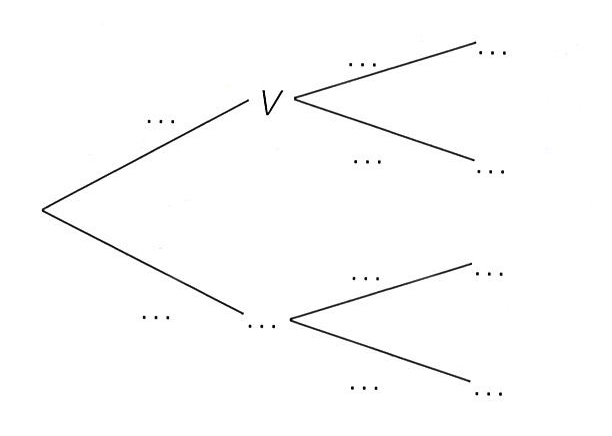
\includegraphics[scale=0.6]{arbre_pond}
	\end{center}

	\begin{solution}
		\begin{center}
			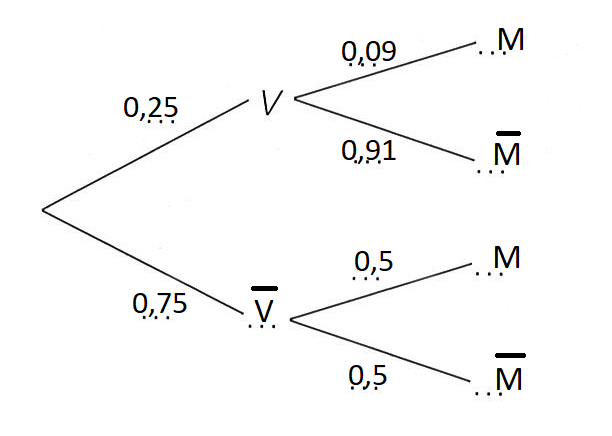
\includegraphics[scale=0.6]{arbre_pond2}
		\end{center}
	\end{solution}

	\question[1] Calculer la probabilité des événements $M \cap V$ et $M \cap \bar{V}$.
	\begin{solution}
		Calcul de $P(M \cap V)$ :
		
		\begin{eqnarray*}
			P(M \cap V) &=& P(V) \times P_V(M) \\
			P(M \cap V) &=& \num{0.25} \times \num{0.09} \\
			P(M \cap V) &=& \num{0.0225}
		\end{eqnarray*}
	
		Calcul de $P(M \cap \bar{V})$ :
		
		\begin{eqnarray*}
			P(M \cap \bar{V}) &=& P(\bar{V}) \times P_{\bar{V}}(M) \\
			P(M \cap \bar{V}) &=& \num{0.75} \times \num{0.5} \\
			P(M \cap \bar{V}) &=& \num{0.375}
		\end{eqnarray*}
	
	La probabilité de l'événement $M \cap V$ est \num{0.0225} et celle de $M \cap \bar{V}$ est \num{0.375}.
	\end{solution}
	
	\question[2] Calculer la probabilité de l'événement $M$ puis de l'événement $\bar{M}$.
	\begin{solution}
		Calcul de $P(M) $ :
		
		\begin{eqnarray*}
			P(M) &=& P(M \cap V) + P(M \cap \bar{V}) \\
			P(M) &=& \num{0.0225} + \num{0.375} \\
			P(M) &=& \num{0.3975}
		\end{eqnarray*}
	
		Calcul de $P(\bar{M}) $ :
		
		\begin{eqnarray*}
			P(\bar{M}) &=& 1 - P(M) \\
			P(\bar{M}) &=& 1 -  \num{0.3975} \\
			P(\bar{M}) &=& \num{0.6025}
		\end{eqnarray*}
	
		La probabilité de l'événement $M$ est \num{0.3975} et celle de $\bar{M}$ est \num{0.6025}.
	\end{solution}
	
	\question[2] Sachant qu'un individu choisi au hasard dans la population n'est pas malade, quelle est la probabilité qu'il ait été vacciné ?
	\begin{solution}
		Calcul de la probabilité qu'un individu soit vacciné sachant qu'il n'est pas malade :
		\begin{eqnarray*}
			P_{\bar{M}}(V) &=& \dfrac{P(V \cap \bar{M})}{P(\bar{M})}\\
			P_{\bar{M}}(V) &=& \dfrac{P(V) \times P_V(\bar{M})}{P(\bar{M})}\\
			P_{\bar{M}}(V) &=& \dfrac{\num{0.25} \times \num{0.91}}{\num{0.6025}}\\
			P_{\bar{M}}(V) &\approx& \num{0.3776}
		\end{eqnarray*}
	
	La probabilité qu'un individu non malade ait été vacciné est \num{0.3776}.
	\end{solution}
\end{questions}  